\documentclass[a4paper,11pt]{article}
\usepackage[top=2cm,bottom=2cm,left=2cm,right=2cm]{geometry}
\usepackage[utf8]{inputenc}
\usepackage[frenchb]{babel}

\usepackage{multirow}
\usepackage{makecell}
\usepackage{fancyhdr}
\usepackage{caption}
\usepackage[final]{pdfpages}
\usepackage{tikz,pgfplots,pgf}
\usepackage{subcaption}
\usepackage{siunitx}
\usepackage[toc,page]{appendix}
\usepackage{tcolorbox, listings} 
\usepackage{sectsty}
\usepackage[french]{minitoc} 
\usepackage{hyperref}
\usepackage{colortbl}
\usepackage{mwe}
\usepackage{amsmath}
\usepackage{lipsum}
\usepackage{enumitem}

\definecolor{Pantone2377C}{HTML}{2C5574}
\definecolor{subtitlecolour}{HTML}{00A2A9}
\definecolor{codegreen}{rgb}{0,0.6,0}
\definecolor{codegray}{rgb}{0.5,0.5,0.5}
\definecolor{codeblue}{HTML}{3E8BC0}
\definecolor{codeorange}{HTML}{ffa334}
\definecolor{backcolour}{HTML}{efefef}

\lstdefinestyle{myPython}{
    language=Python,
    backgroundcolor=\color{backcolour},   
    commentstyle=\color{codegreen},
    otherkeywords={plt, np, df},
    keywordstyle=\color{codeblue},
    numberstyle=\tiny\color{codegray},
    stringstyle=\color{codeorange},
    basicstyle=\ttfamily\footnotesize,
    breakatwhitespace=false,         
    breaklines=true,                 
    keepspaces=true,                 
    numbers=left,       
    numbersep=5pt,                  
    showspaces=false,                
    showstringspaces=false,
    showtabs=false,                  
    tabsize=2,
    inputencoding=utf8
}

\lstdefinestyle{myLog}{
    backgroundcolor=\color{backcolour},   
    basicstyle=\ttfamily\footnotesize,
    breakatwhitespace=false,         
    breaklines=true,                 
    keepspaces=true,                 
    numbers=left,       
    numbersep=5pt,                  
    showspaces=false,                
    showstringspaces=false,
    showtabs=false,                  
    tabsize=2,
    inputencoding=utf8
}

\lstset{
  backgroundcolor=\color{backgroundColour},   
  commentstyle=\color{codegreen},
  keywordstyle=\color{codeblue},
  numberstyle=\tiny\color{codegray},
  stringstyle=\color{codeorange},
  basicstyle=\footnotesize,
  breakatwhitespace=false,         
  breaklines=true,                 
  captionpos=b,                    
  keepspaces=true,                 
  numbers=left,                    
  numbersep=5pt,                  
  showspaces=false,                
  showstringspaces=false,
  showtabs=false,                  
  tabsize=2,
  literate=
  {é}{{\'e}}1
  {è}{{\`{e}}}1
  {ê}{{\^{e}}}1
  {û}{{\^{u}}}1
  {ù}{{\`{u}}}1
  {â}{{\^{a}}}1
  {à}{{\`{a}}}1
  {ç}{{\c{c}}}1
  {Ç}{{\c{C}}}1
  {ô}{{\^{o}}}1
}


% Entête et pied de page
\pagestyle{fancy}
\rhead{
\includegraphics [scale=0.035]{img/ensta-logo.png}}
\chead{}
\lhead{}
\lfoot{Tanguy ROUDAUT - Tadios QUINIO}
\rfoot{FIPA promotion 2024}
\cfoot{\thepage}
\renewcommand{\headrulewidth}{0.4pt}
\renewcommand{\footrulewidth}{0.4pt}


\title{TP3: Intervalle de confiance}
\author{Tanguy ROUDAUT — Tadios QUINIO \and FIPASE 24}
\date{22 Septembre 2022}

\begin{document}

\maketitle

\section{Dissection d’une gaussienne}
\vspace{.2cm}

\noindent
Données mesurées : 0.82 0.87 0.77 0.96 0.75 0.83 0.87 0.81

%%%%%
\begin{itemize}[label={},itemindent=-2em,leftmargin=2em]
    \item \textbf{Question~1~:} Considérant que l’échantillon a été engendré par une loi gaussienne, donner un intervalle
    de confiance pour son espérance. On utilisera les fonctions tinv, mean et var ou std/t.ppf, np.mean,
    np.std. Préciser toutes les hypothèses que vous retenez.
\end{itemize}
\vspace{.2cm}

\noindent
Dans cette question, l'échantillon est de longueur~$n=8$. \\
Si un échantillon est de longueur~$n<30$ avec une $\sigma^{2}$ inconnu, il faut utiliser le cas suivant~: 
\textit{Intervalles de confiance de la moyenne d’une distribution normale, $\sigma^{2}$ inconnue} \\

\noindent
Ce qui nous amène à utiliser les formules \ref*{eq:ic_normale_inf} et \ref*{eq:ic_normale_sup} pour déterminer l'intervalle de confiance $[I, u]$. 

\begin{figure}[!h]
    \centering
    \begin{minipage}{.48\linewidth}
        \begin{equation}
            I = \overline{X_{n}} - t_{n-1,\frac{\alpha}{2}} \frac{S_{n-1}}{\sqrt{n}}
            \label{eq:ic_normale_inf}
        \end{equation}
    \end{minipage}\hfill\vline
    \begin{minipage}{.48\linewidth}
        \begin{equation}
            u = \overline{X_{n}} + t_{n-1,\frac{\alpha}{2}} \frac{S_{n-1}}{\sqrt{n}}
            \label{eq:ic_normale_sup}
        \end{equation}
    \end{minipage}
\end{figure}

\noindent
Comme $\sigma^{2}$ est inconnue, on peut l'approcher par $S_{n-1}^{2}$ puis en déduire $S_{n-1}$. \\
On peut également rappeler que $t_{n-1,\frac{\alpha}{2}}$ est le quantile d’ordre $\frac{\alpha}{2}$ d’une loi de Student de $n - 1$ degrés de liberté, déterminable en python avec \textit{scipy.stats.t.ppf()}.

\vspace{.2cm}


\begin{lstlisting}[style=myPython, caption=Code Python question 1, frame=lines]
x = np.array([0.82, 0.87, 0.77, 0.96, 0.75, 0.83, 0.87, 0.81])
xn = np.mean(x)
ecart_type_x = np.std(x, ddof=1)
n = len(x)
ic = 95
alpha = 1 - ic / 100
t = stats.t.ppf(1 - (alpha / 2), n - 1)

I = xn - (t * ecart_type_x) / np.sqrt(n)
u = xn + (t * ecart_type_x) / np.sqrt(n)

I = round(I, 3)
u = round(u, 3)

print("Borne inférieur:", I, "\n", "Borne supérieur:", u)
\end{lstlisting}

\begin{lstlisting}[style=myLog, caption=Résultat du code, frame=lines]
Borne inférieur: 0.779 
Borne supérieur: 0.890
\end{lstlisting}

\noindent
On peut donc conclure qu'il y'a $95\%$ de chance que l'espérance ce trouve dans l'intervalle $[0,779; 0,890]$.

\vspace{.5cm}

\clearpage

%%%%%
\begin{itemize}[label={},itemindent=-2em,leftmargin=2em]
    \item \textbf{Question~2~:} Les données sont maintenant [0.84 0.87 0.89 0.73 0.84 0.81 0.88 0.85 0.89 0.79 0.79 0.90
    0.59 0.75 0.67 0.76 0.86 0.88 0.70 0.75 0.81 0.77 0.83 0.84 0.71 0.78 0.59 0.91 0.74 0.68 0.77 0.66
    0.80 0.74 1.02 0.91 0.55 0.84 0.66 0.77]. Considérant que l’échantillon a été engendré par une
    loi gaussienne, donner un intervalle de confiance pour son espérance. On utilisera les fonctions
    (norminv, mean et var ou std ou norm.ppf, np.mean, np.std). Préciser toutes les hypothèses que
    vous retenez. Quel est dans ce cas, l’intérêt de la loi gaussienne~?
\end{itemize}
\vspace{.2cm}

\noindent
Dans cette question l'échantillon est de longueur~$n=40$. \\
Pour un échantillon de longueur~$n>30$ suivant une distribution normale centrée réduite~$\mathcal{N}(0,\,1)$ avec $\sigma^{2}$ inconnu, il faut utiliser le cas suivant~: 
\textit{Intervalle de confiance de la moyenne d’une distribution dans le cas d’un grand échantillon} \\

\noindent
Ce qui nous amène à utiliser la formule~\ref*{eq:ic_grand1} pour déterminer l'intervalle de confiance.

\begin{equation}
    \hat{p} - z_{\frac{\alpha}{2}} \sqrt{\frac{S_{n-1}}{n}} \leq p \leq \hat{p} + z_{\frac{\alpha}{2}} \sqrt{\frac{S_{n-1}}{n}}
    \label{eq:ic_grand1}
\end{equation}

\begin{center}
    avec \qquad $z_{\frac{\alpha}{2}}=erf^{-1}(1 - \frac{\alpha}{2})$ \qquad et \qquad $\alpha = 1- \frac{IC\%}{100}$
\end{center}

\noindent
Comme $\sigma^{2}$ est inconnue, on peut l'approcher par $S_{n-1}^{2}$ puis en déduire $S_{n-1}$. \\
On peut également rappeler que $z_{\frac{\alpha}{2}}$ peut être déterminé avec la table et en python avec \textit{stats.norm.ppf()}.

\vspace{.2cm}

\begin{lstlisting}[style=myPython, caption=Code Python question 2, frame=lines]
x = np.array([0.84, 0.87, 0.89, 0.73, 0.84, 0.81, 0.88, 0.85, 0.89, 0.79, 0.79, 0.90,
              0.59, 0.75, 0.67, 0.76, 0.86, 0.88, 0.70, 0.75, 0.81, 0.77, 0.83, 0.84, 
              0.71, 0.78, 0.59, 0.91, 0.74, 0.68, 0.77, 0.66, 0.80, 0.74, 1.02, 0.91,
              0.55, 0.84, 0.66, 0.77])

p = np.mean(x)
ecart_type_x = np.std(x, ddof=1)
n = len(x)
ic = 95
alpha = 1 - ic / 100
z = stats.norm.ppf(1 - (alpha / 2), loc=0, scale=1)

borne_inf = p - z * (ecart_type_x/np.sqrt(n))
borne_supp = p + z * (ecart_type_x/np.sqrt(n))

borne_inf = round(borne_inf, 3)
borne_supp = round(borne_supp, 3)

print("Borne inférieur:", borne_inf, "\n", "Borne supérieur:", borne_supp)
\end{lstlisting}

\begin{lstlisting}[style=myLog, caption=Résultat du code, frame=lines]
Borne inférieur: 0.755 
Borne supérieur: 0.816
\end{lstlisting}


\noindent
On peut donc conclure qu'il y'a $95\%$ de chance que l'espérance ce trouve dans l'intervalle $[0,755; 0,816]$

\vspace{.5cm}


\clearpage

\section{Recoder l’exercice~4 du TD~: sondages}
\vspace{.2cm}

\noindent
À la veille d’une consultation électorale, nous effectuons un sondage. 


%%%%%
\begin{itemize}[label={},itemindent=-2em,leftmargin=2em]
    \item \textbf{Question~3~:} Dans un échantillon représentatif de 1000~personnes, 500~personnes déclarent vouloir
    voter pour Dupond, 250 pour Durand et 50 pour Duroc. Donner les intervalles de confiance à $95\%$
    et $99\%$ du pourcentage de personnes ayant l’intention de voter Dupond, Durand ou Duroc.
\end{itemize}
\vspace{.2cm}


\noindent
Formules utilisées~:

\begin{equation}
    \hat{p} - z_{\frac{\alpha}{2}} \sqrt{\frac{\hat{p}(1-\hat{p})}{n}} \leq p \leq \hat{p} + z_{\frac{\alpha}{2}} \sqrt{\frac{\hat{p}(1-\hat{p})}{n}}
    \label{eq:ic_grand2}
\end{equation}

\begin{center}
    avec \qquad $z_{\frac{\alpha}{2}}=erf^{-1}(1 - \frac{\alpha}{2})$ \qquad et \qquad $\alpha = 1- \frac{IC\%}{100}$
\end{center}

\vspace{.2cm}

\begin{lstlisting}[style=myPython, caption=Code Python question 3, frame=lines]
n = 1000
n_dupond = 500
n_durand = 250
n_duroc = 50

def intervalle_confiance(n, x, ic ):
    p = x/n
    alpha = 1 - ic / 100
    z = stats.norm.ppf(1 - (alpha / 2), loc=0, scale=1)
    borne_inf = p - z * (np.sqrt(p*(1-p)/n))
    borne_supp = p + z * (np.sqrt(p*(1-p)/n))

    return round(borne_inf, 3), round(borne_supp, 3)

borne_inf_dupond_95, borne_supp_dupond_95 = intervalle_confiance(n, n_dupond, 95)
borne_inf_durand_95, borne_supp_durand_95 = intervalle_confiance(n, n_durand, 95)
borne_inf_duroc_95, borne_supp_duroc_95 = intervalle_confiance(n, n_duroc, 95)
borne_inf_dupond_99, borne_supp_dupond_99 = intervalle_confiance(n, n_dupond, 99)
borne_inf_durand_99, borne_supp_durand_99 = intervalle_confiance(n, n_durand, 99)
borne_inf_duroc_99, borne_supp_duroc_99 = intervalle_confiance(n, n_duroc, 99)

print(" Dupond")
print("\t --> Borne inférieur à 95%:", borne_inf_dupond_95)
print("\t --> Borne supérieur à 95%:", borne_supp_dupond_95)
print("\t\t\t ------------------------")
print("\t --> Borne inférieur à 99%:", borne_inf_dupond_99)
print("\t --> Borne supérieur à 99%:", borne_supp_dupond_99)
print(" Durand")
print("\t --> Borne inférieur à 95%:", borne_inf_durand_95)
print("\t --> Borne supérieur à 95%:", borne_supp_durand_95)
print("\t\t\t ------------------------")
print("\t --> Borne inférieur à 99%:", borne_inf_durand_99)
print("\t --> Borne supérieur à 99%:", borne_supp_durand_99)
print(" Duroc")
print("\t --> Borne inférieur à 95%:", borne_inf_duroc_95)
print("\t --> Borne supérieur à 95%:", borne_supp_duroc_95)
print("\t\t\t ------------------------")
print("\t --> Borne inférieur à 99%:", borne_inf_duroc_99)
print("\t --> Borne supérieur à 99%:", borne_supp_duroc_99, end="\n\n")
\end{lstlisting}

\begin{lstlisting}[style=myLog, caption=Résultat du code, frame=lines]
Dupond
    --> Borne inférieur à 95%: 0.469
    --> Borne supérieur à 95%: 0.531
        ------------------------
    --> Borne inférieur à 99%: 0.459
    --> Borne supérieur à 99%: 0.541
Durand
    --> Borne inférieur à 95%: 0.223
    --> Borne supérieur à 95%: 0.277
        ------------------------
    --> Borne inférieur à 99%: 0.215
    --> Borne supérieur à 99%: 0.285
Duroc
    --> Borne inférieur à 95%: 0.036
    --> Borne supérieur à 95%: 0.064
        ------------------------
    --> Borne inférieur à 99%: 0.032
    --> Borne supérieur à 99%: 0.068
\end{lstlisting}

\vspace{.5cm}


%%%%%
\begin{itemize}[label={},itemindent=-2em,leftmargin=2em]
    \item \textbf{Question~4~:} Nous évaluons le pourcentage de personnes ayant l’intention de voter pour un quatrième
    candidat, Duval, à $17\%$. Combien faut-il interroger de personnes pour obtenir une précision de
    $1\%$ pour l’intervalle de confiance (à $95\%$) de la proportion de personnes ayant l’intention de voter
    Duval~?
\end{itemize}
\vspace{.2cm}

\begin{equation}
    n = \left( \sqrt{\frac{Z_{\alpha/2}}{E}} \right)^{2} \hat{p}(1 - \hat{p}) \qquad \text{avec $E$ = erreur = précision}
    \label{eq:n}
\end{equation}

\vspace{.2cm}

\begin{lstlisting}[style=myPython, caption=Code Python question 4, frame=lines]
ic = 95
alpha = 1 - ic / 100
p = 17/100
err = 1/100
z = stats.norm.ppf(1 - (alpha / 2), loc=0, scale=1)
n = (z/err)**2 * p*(1-p)
n = np.ceil(n)

print("Nombre de personne à intérroger:", n, end='\n\n')
\end{lstlisting}

\begin{lstlisting}[style=myLog, caption=Résultat du code, frame=lines]
Nombre de personne à intérroger: 5421.0
\end{lstlisting}

\vspace{.5cm}

\section{Dommage de casques}
\vspace{.2cm}

\noindent
Un échantillon aléatoire de 50~casques de motos et de courses automobiles a été testé à l’impact. Des
dommages ont été observés pour 18 d’entre eux. 

%%%%%
\begin{itemize}[label={},itemindent=-2em,leftmargin=2em]
    \item \textbf{Question~5~:} Construire un intervalle de confiance à $95\%$ pour la vraie proportion des casques qui
    montreraient des dommages à ce test.
\end{itemize}
\vspace{.2cm}

\noindent
Pour répondre à cette question nous avons utilisé la formule~\ref*{eq:ic_grand2}, pour le code python on a utiliser la fonction 
\textit{intervalle\_confiance(n, x, ic)} réalisé à la question~3.

\vspace{.2cm}


\begin{lstlisting}[style=myPython, caption=Code Python question 5, frame=lines]
n_casques = 50
n_dommages = 18
borne_inf_dommages_95, borne_supp_dommages_95 = intervalle_confiance(n_casques, n_dommages, 95)

print("Casques endommagés")
print("\t --> Borne inférieur à 95%:", borne_inf_dommages_95)
print("\t --> Borne supérieur à 95%:", borne_supp_dommages_95, end="\n\n")
\end{lstlisting}

\begin{lstlisting}[style=myLog, caption=Résultat du code, frame=lines]
Casques endommagés
    --> Borne inférieur à 95%: 0.227
    --> Borne supérieur à 95%: 0.493
\end{lstlisting}



\vspace{.5cm}


%%%%%
\begin{itemize}[label={},itemindent=-2em,leftmargin=2em]
    \item \textbf{Question~6~:} En utilisant un estimateur ponctuel de p à partir de 50~casques, combien de casques
    doivent être testés pour avoir une erreur inférieure à 0,02 pour l’IC à $95\%$ de la proportion p~?
\end{itemize}
\vspace{.2cm}

\noindent
Pour répondre à cette question, nous avons utilisé la formule \ref*{eq:n} \textit{(cf. Question~4)}.

\vspace{.2cm}


\begin{lstlisting}[style=myPython, caption=Code Python question 6, frame=lines]
ic = 95
alpha = 1 - ic / 100
p = 18/50
err = .02
z = stats.norm.ppf(1 - (alpha / 2), loc=0, scale=1)
n = (z/err)**2 * p*(1-p)
n = np.ceil(n)

print("Nombre de casque à tester:", n, end='\n\n')
\end{lstlisting}

\begin{lstlisting}[style=myLog, caption=Résultat du code, frame=lines]
Nombre de casque à tester: 2213.0
\end{lstlisting}

\vspace{.5cm}


%%%%%
\begin{itemize}[label={},itemindent=-2em,leftmargin=2em]
    \item \textbf{Question~7~:} Quelle doit être la taille de l’échantillon pour obtenir une erreur inférieure à 0,02 pour
    l’IC à $95\%$ de la proportion $p$. Vous considérerez que vous ne connaissez ni la valeur de $p$ ni celle
    de $\hat{p}$~? Vous déterminerez la valeur $p$ pour que la fonction $n=f(p)$ soit maximale.
\end{itemize}

\begin{figure}[!h]
    \centering
    \begin{minipage}{.48\linewidth}
        En théorie le cas le plus défavorable a lieu quand $p=0.5$ (soit $n$ maximale), mais pour répondre à la question et vérifier cette théorie nous avons décidé de créer un vecteur $p$, contenant des valeurs de 0 à 1 par pas de 0,1. En calculant $n$ avec les différentes valeurs de $p$, nous pouvons obtenir 
        la valeur max de $n$ avec la fonction \textit{max}. \\

        Pour illustrer et vérifier la valeur obtenue, on a tracé la fonction $n=f(p)$ et la valeur max obtenue, on trouve bien une valeur de $p=0.5$ \textit{(cf. Figure~\ref*{fig:figure1})}.
    \end{minipage}\hfill
    \begin{minipage}{.48\linewidth}
        \begin{center}
            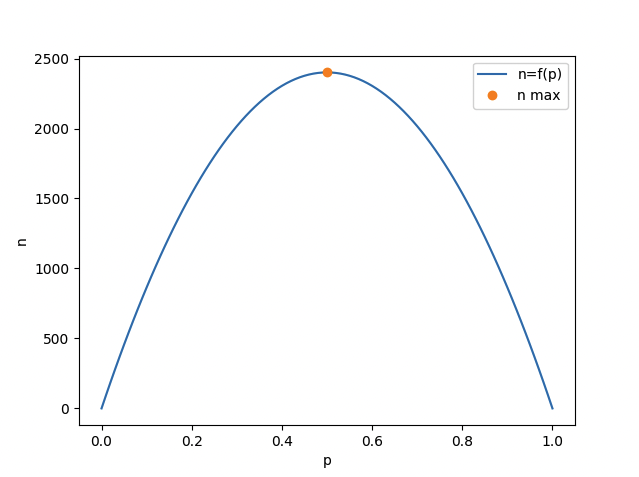
\includegraphics[width=1\textwidth]{img/figure1.png}
            \caption{\label{fig:figure1}Courbe de $n=f(p)$}
        \end{center}
    \end{minipage}
\end{figure}

\noindent
Nous avons utilisé la formule \ref*{eq:n} \textit{(cf. Question~4)}.

\vspace{.2cm}


\begin{lstlisting}[style=myPython, caption=Code Python question 7, frame=lines]
ic = 95
alpha = 1 - ic / 100
err = .02
z = stats.norm.ppf(1 - (alpha / 2), loc=0, scale=1)
p = np.linspace(0, 1, 101)
n = (z/err)**2 * p*(1-p)
index_n_max = np.where(n == max(n))
n = np.ceil(float(n[index_n_max]))

print("Question 7:\n", "Nombre de casque à tester:", n, end='\n\n')
\end{lstlisting}

\begin{lstlisting}[style=myLog, caption=Résultat du code, frame=lines]
Nombre de casque à tester: 2401.0
\end{lstlisting}


\section{Code complet}
\begin{lstlisting}[style=myPython, caption=Code Python complet TP3, frame=lines]
from scipy import stats
import numpy as np

# question 1
x = np.array([0.82, 0.87, 0.77, 0.96, 0.75, 0.83, 0.87, 0.81])
xn = np.mean(x)
ecart_type_x = np.std(x, ddof=1)
n = len(x)
ic = 95
alpha = 1 - ic / 100
t = stats.t.ppf(1 - (alpha / 2), n - 1)

I = xn - (t * ecart_type_x) / np.sqrt(n)
u = xn + (t * ecart_type_x) / np.sqrt(n)

I = round(I, 3)
u = round(u, 3)

print("Question 1:\n", "Borne inférieur:", I, "\n", "Borne supérieur:", u, end="\n\n")

# question 2
x = np.array([0.84, 0.87, 0.89, 0.73, 0.84, 0.81, 0.88, 0.85, 0.89, 0.79, 0.79, 0.90,
              0.59, 0.75, 0.67, 0.76, 0.86, 0.88, 0.70, 0.75, 0.81, 0.77, 0.83, 0.84, 
              0.71, 0.78, 0.59, 0.91, 0.74, 0.68, 0.77, 0.66, 0.80, 0.74, 1.02, 0.91,
              0.55, 0.84, 0.66, 0.77])
p = np.mean(x)
ecart_type_x = np.std(x, ddof=1)
n = len(x)
ic = 95
alpha = 1 - ic / 100
z = stats.norm.ppf(1 - (alpha / 2), loc=0, scale=1)

borne_inf = p - z * (ecart_type_x/np.sqrt(n))
borne_supp = p + z * (ecart_type_x/np.sqrt(n))

borne_inf = round(borne_inf, 3)
borne_supp = round(borne_supp, 3)

print("Question 2:\n", "Borne inférieur:", borne_inf, "\n", "Borne supérieur:", borne_supp, end="\n\n")

# question 3
n = 1000
n_dupond = 500
n_durand = 250
n_duroc = 50

def intervalle_confiance(n, x, ic ):
    p = x/n
    alpha = 1 - ic / 100
    z = stats.norm.ppf(1 - (alpha / 2), loc=0, scale=1)
    borne_inf = p - z * (np.sqrt(p*(1-p)/n))
    borne_supp = p + z * (np.sqrt(p*(1-p)/n))

    return round(borne_inf, 3), round(borne_supp, 3)

borne_inf_dupond_95, borne_supp_dupond_95 = intervalle_confiance(n, n_dupond, 95)
borne_inf_durand_95, borne_supp_durand_95 = intervalle_confiance(n, n_durand, 95)
borne_inf_duroc_95, borne_supp_duroc_95 = intervalle_confiance(n, n_duroc, 95)
borne_inf_dupond_99, borne_supp_dupond_99 = intervalle_confiance(n, n_dupond, 99)
borne_inf_durand_99, borne_supp_durand_99 = intervalle_confiance(n, n_durand, 99)
borne_inf_duroc_99, borne_supp_duroc_99 = intervalle_confiance(n, n_duroc, 99)

print("Question 3:")
print(" Dupond")
print("\t --> Borne inférieur à 95%:", borne_inf_dupond_95)
print("\t --> Borne supérieur à 95%:", borne_supp_dupond_95)
print("\t\t\t ------------------------")
print("\t --> Borne inférieur à 99%:", borne_inf_dupond_99)
print("\t --> Borne supérieur à 99%:", borne_supp_dupond_99)
print(" Durand")
print("\t --> Borne inférieur à 95%:", borne_inf_durand_95)
print("\t --> Borne supérieur à 95%:", borne_supp_durand_95)
print("\t\t\t ------------------------")
print("\t --> Borne inférieur à 99%:", borne_inf_durand_99)
print("\t --> Borne supérieur à 99%:", borne_supp_durand_99)
print(" Duroc")
print("\t --> Borne inférieur à 95%:", borne_inf_duroc_95)
print("\t --> Borne supérieur à 95%:", borne_supp_duroc_95)
print("\t\t\t ------------------------")
print("\t --> Borne inférieur à 99%:", borne_inf_duroc_99)
print("\t --> Borne supérieur à 99%:", borne_supp_duroc_99, end="\n\n")

# question 4
ic = 95
alpha = 1 - ic / 100
p = 17/100
err = 1/100
z = stats.norm.ppf(1 - (alpha / 2), loc=0, scale=1)
n = (z/err)**2 * p*(1-p)
n = np.ceil(n)

print("Question 4:\n", "Nombre de personne à intérroger:", n, end='\n\n')

# question 5
n_casques = 50
n_dommages = 18
borne_inf_dommages_95, borne_supp_dommages_95 = intervalle_confiance(n_casques, n_dommages, 95)

print("Question 5:")
print(" Casques endommagés")
print("\t --> Borne inférieur à 95%:", borne_inf_dommages_95)
print("\t --> Borne supérieur à 95%:", borne_supp_dommages_95, end="\n\n")

# question 6
ic = 95
alpha = 1 - ic / 100
p = 18/50
err = .02
z = stats.norm.ppf(1 - (alpha / 2), loc=0, scale=1)
n = (z/err)**2 * p*(1-p)
n = np.ceil(n)

print("Question 6:\n", "Nombre de casque à tester:", n, end='\n\n')

# question 7
ic = 95
alpha = 1 - ic / 100
err = .02
z = stats.norm.ppf(1 - (alpha / 2), loc=0, scale=1)
p = np.linspace(0, 1, 101)
n = (z/err)**2 * p*(1-p)
index_n_max = np.where(n == max(n))
n = np.ceil(float(n[index_n_max]))

print("Question 7:\n", "Nombre de casque à tester:", n, end='\n\n')    
\end{lstlisting}



\end{document}